% !TEX root = ../mechatronics.tex
\chapter{Linear Systems Theory}\label{chp:linearsystems}

Linear systems theory is fundamental to understanding,  analyzing and designing engineering systems. This chapter introduces some essential concepts and tools employed in linear systems theory. We will only present mathematical formulations and results without proofs or any detailed explanations.

\section{Linear Systems}
In the engineering context, a system is a collection of components that interact to perform a specific function. When we think of a system we usually think of a block that has inputs and outputs; the components of the system, their interconnections and interactions are all abstracted away in the block as shown in Figure~\ref{fig:04-01-system}. This system has three inputs, $u_1$, $u_2$, and $u_3$, and two outputs, $y_1$ and $y_2$. 
\begin{figure}[htbp]
    \centering
    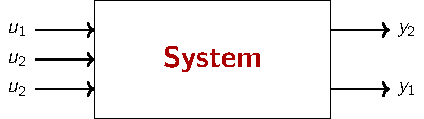
\includegraphics[width=0.5\textwidth]{figures/ch04/fig04-01.pdf}
    \caption{Block diagram representation of a system with three inputs and two outputs.}
    \label{fig:04-01-system}
\end{figure}
The inputs are signals that can influence the internal behavior and/or output of the system, and the outputs are the readouts of the internal state of the system and the current input. This abstraction allows engineers to analyze and design complex systems without needing to understand every detail of their internal workings. In this type of characterization, we are simply interested in the relationship between the inputs and outputs of the system without worrying about the internal details.

When a system has a single input and a single output, like most systems you learn in an undergraduate signal processing or control theory course, it is referred to as a \textbf{single-input single-output} (SISO) system. When a system has multiple inputs and multiple outputs, like the one shown in Figure~\ref{fig:04-01-system}, it is referred to as a \textbf{multiple-input multiple-output} (MIMO) system. For most of this chapter, will will present ideas for SISO linear system, but extend these to MIMO systems later.

A SISO system $\mathcal{H}$ is said to be \textit{linear} if it satisfies the following two properties for all inputs $u(t)$ and outputs $y(t)$, and all scalars $\alpha$:
\begin{itemize}
    \item \textbf{Homogeneity (or scaling)}: If $u(t)$ is an input to the system $\mathcal{H}$ and $y(t)$ is the corresponding output, then for any scalar $\alpha$, the input $\alpha u(t)$ produces the output $\alpha y(t)$.
    \begin{equation}
        \mathcal{H}(\alpha u(t)) = \alpha \mathcal{H}(u(t))
        \label{eq:04-01-homogeneity}
    \end{equation}
    \item \textbf{Additivity}: If $u(t)$ and $v(t)$ are inputs to the system $\mathcal{H}$ with corresponding outputs $y_u(t)$ and $y_v(t)$, then the input $u(t) + v(t)$ produces the output $y_u(t) + y_v(t)$.
    \begin{equation}
        \mathcal{H}(u(t) + v(t)) = \mathcal{H}(u(t)) + \mathcal{H}(v(t))
        \label{eq:04-02-additivity}
    \end{equation}
\end{itemize}
Effectively, the scaling factor $\alpha$ (in Eq.~\ref{eq:04-01-homogeneity}) and the addition operation (in Eq.~\ref{eq:04-02-additivity}) can be factored out of the paranthesis. This is the simplicity offered by the linearity assumption. These two properties together give us the superposition principle,
\begin{equation}
    \mathcal{H}(\alpha_1 u_1(t) + \alpha_2 u_2(t)) = \alpha_1 \mathcal{H}(u_1(t)) + \alpha_2 \mathcal{H}(u_2(t))
    \label{eq:04-03-superposition}
\end{equation}
for any inputs $u_1(t)$ and $u_2(t)$ and scalars $\alpha_1$ and $\alpha_2$. This means that the response of a linear system to a linear combination of inputs is the same linear combination of the responses to each input. This means that once we know the output of the system for two inputs for a linear system, we automatically know the output for any linear combination of those two inputs.

\begin{boxedstuff}
    \begin{problem}
        Verify that the system $y(t) = \mathcal{H}\left(u(t)\right) = 5 \cdot u(t)$ is linear. Whereas the systems, $y(t) = \mathcal{H}\left(u(t)\right) = 3 \cdot u^2(t)$ and $y(t) = \mathcal{H}\left(u(t)\right) = u(t) + 1$ are not.
    \end{problem}
\end{boxedstuff}
The extension to MIMO systems is straightforward: a MIMO system is linear if it satisfies the homogeneity and additivity properties for all inputs and outputs, where the inputs and outputs are vectors.

Linearity is a strict or highly constraining assumption. For most systems the linearity assumption hold for a restricted range of inputs and output. For instance, a practical resistor from the lab can be very well approximated as a linear system with votlage across it as the input and the current through it as the output for small values of voltage and current, i.e. as long as it is operated well within the power ratings of the resistor. It will not be linear for large voltages and currents. 

\section{Time-invariant systems}
A system whose behavior or input-output relationship does not change with time is called a time-invariant system. If my new computer is time-invariant, this essentially means that my computer will continue to behave like a new computer for all time. Like the linearity assumption, for most systems time-invariance would hold over finite durations of time, but not beyond that. My computer might person as well as it did when I bought for a couple of years but may be not beyond that. Mathematically, a system $\mathcal{H}$ is time-invariant if and only if the folloowing hold for all inputs and all time,
\begin{equation}
    y\left(t\right) = \mathcal{H}\left(u\left(t\right)\right) \implies y\left(t - T\right) = \mathcal{H}\left(u\left(t - T\right)\right), \,\,\, \forall \, u(t) \, \text{ and } \, T
    \label{eq:04-04-time-inv}
\end{equation}
In the above equation, it looks like we have simply replaced $t$ by $t-T$, but the issue a bit more subtle. The above equation means that if $y(t)$ is the output of the system to the input $u(t)$ at present, then if I apply the the same input at some point in the future or if I had applied it at some time in the past, the system's output would be exact the same the one at present, except that it appears in the future or the past, respectively.

A system that is both linear and time-invariant is called a linear time-invaraint (LTI) system, which is an important class of systems in engineering. Continuous-time LTI systems can be described by linear constant coefficient ordinary differential equations (ODEs) or linear constant coefficient difference equations in the discrete-time case.

\section{Impulse response and convolution}
We said earlier that if we know the output of a linear system to one or more inputs, then we can easily compute the output of the system for any linear combination of these inputs. It turns out that there is a special input signal that is very useful for characterizing LTI systems. It is the Dirac delta function or the impulse function $\delta\left(t\right)$ in the continuous-time case and the Kronecker delta function $\delta\left[n\right]$ in the discrete-time case. We will first look at the continuous-time case. The Dirac delta function $\delta$ is not a function in the traditional sense, but rather a distribution. It is defined by the following property
\begin{equation}
    \int_{-\infty}^{\infty} \delta\left(t\right) \, dt = 1 \quad \text{and} \quad \int_{-\infty}^{\infty} x\left(t\right)\delta\left(t - t_0\right) \, dt = x\left(t_0\right)
    \label{eq:04-05-delta-ct}
\end{equation}